

Machine learning (ML) is part of artificial intelligence (AI). as shown in Fig.~\ref{fig:ML_diagram}
AI is the process of computers being trained to mimic the human brain in how it learns and solves problems.
There are two types of learning: ML learning where it needs human intervene, and deep learning (DL) which is a subset of ML where computers learn from its own errors.  

ML is algorithms, collection of tools and techniques, with the ability to learn without being explicitly programmed, more data better decisions.

ML algor could be categorized into two main groups depending on the data used in training the machine learning model: supervised learning, using labeled data (target) and unsupervised learning.

There are dozens of different ML methods (algorithms) that could be used depending on the problem we want to solve either to classify things (classification problem) or make quantitative predictions (regression problem).
Both of these problems are supervised leaning.

ML model is the result of running a ML algorithm on data. It contains the model data and prediction algorithm. 

Various python-based libraries such as schitkit-learn, TensorFlow, keras are used tools for ML algorithms and model implementation.  

\begin{figure}[t!]
\centering
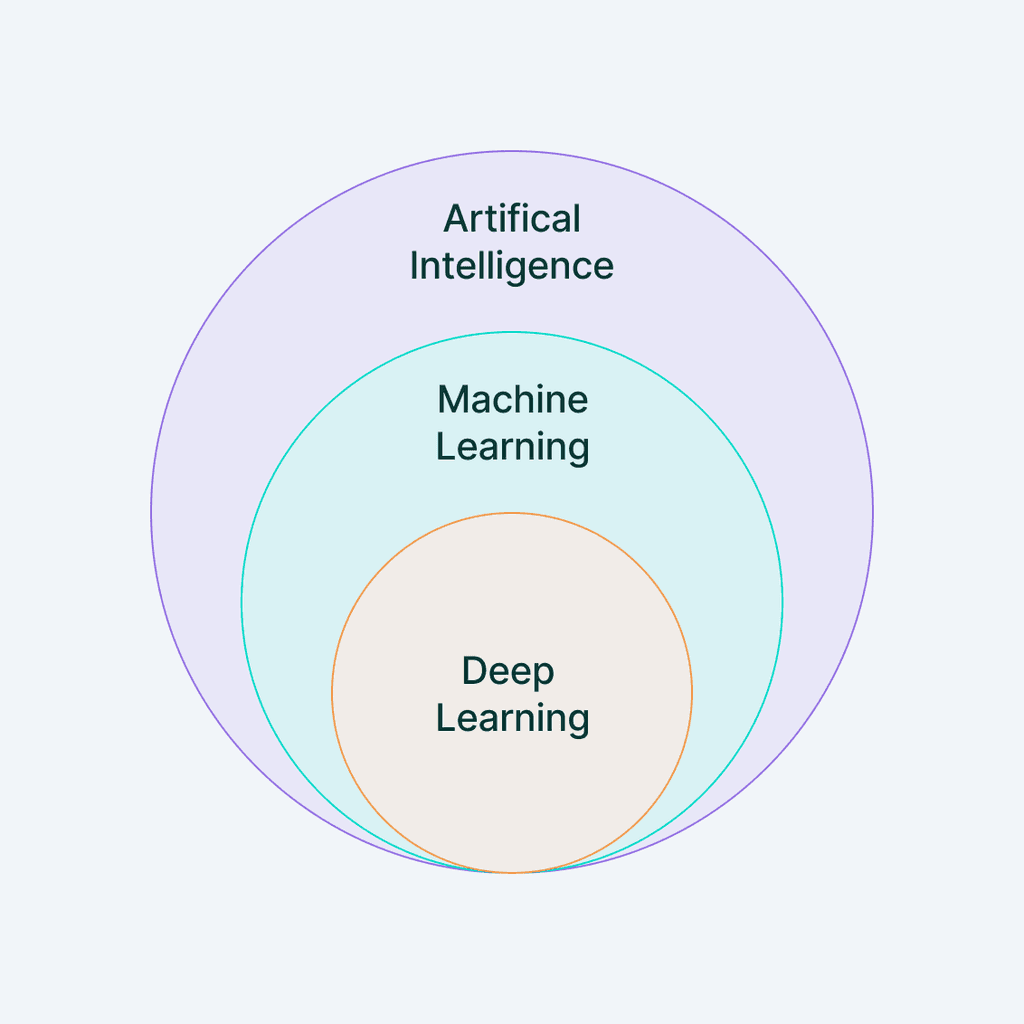
\includegraphics[width=0.99\textwidth]{figures/ML_diagram.png}
\caption[ML and AI]{}. Figure source~\cite{SMtable}.
\label{fig:ML_diagram}}                                                                                                                                                                                        
\end{figure}
  
\subsection{BDT}

Decision tree: is a tool that could be used to divide the data into simple regions in order to classify or regress the inputs. In (regression tasks): the model predicts the numerical value of the target. ML method based on decision trees uses a large number of these trees to classify or regress to a true output.

boosted decision trees (BDTs) : when the outputs of the trees in the method are dependent on one another.  types of boosting available to BDTs: adaptive boosting (adaBoost), gradient boosting, extreme gradient boosting (XGBoost) which is what is implemented here. (Quickly mention the difference between them)

Gradient boosting (GB): based on popular optimization technique called gradient descent algorithm. same concept but instead of minimizing the output function, it minimizes the error function/ loss in the direction of the process. So here New prediction (GB) = old prediction + learning rate * residual. <= this shows that the total predictive model is just a collection of all trees in the model. (Check written notes for a better way to explain GB)

Extreme Gradient boosting (XGB): is an advance version of the GB. to avoid the overfitting penalty terms are added to the residual of GB. So here new prediction (XGB) = old prediction (GB) + penalty * residual(branch) = mean/median of the error of the current branch.

Where learning rate: the size of the steps of the gradient descent. And error/residual of the decision making: true output - prediction made by the model. 


\subsection{NN} 

Neural Networks are one of the most used ML algorithms. The simplest NN contains an input, output, one hidden layer. if the NN has more one hidden layer is called Deep NN. (insert picture of NN) (check written notes for more details on how basic network training is done generally, forward propagation, backpropagation)  

% GNN
GNN is a type of NN that is used to process data that can be represented as graphs. comparing to some kinds of NN, GNN can be applied on sparse data. 

graph consists of nodes (features of the objects, meaning in our case will be represented by rechits) and edges (reflect the relationship between the rechit, in our case seeing how rechits are connected, in clusters that represent one particle). information in GNN can be shared between neighbors. 

the vector feature of each node is transformed into messages (using dense layers) that will be sent to the neighbors (message passing) in this way each node will learn about its neighbors and itself. (add picture that shows massage passing)


